% ============================================================
%  BioPhasor: Phasor Based Cellular Dynamics and Multi-Omics Integration
%  Research-paper format (REVTeX 4-2).
% ============================================================
\documentclass[preprint,12pt,amsmath,amssymb,superscriptaddress,floatfix]{revtex4-2}

% --- Packages ---
\usepackage[T1]{fontenc}
\usepackage{amsmath, amssymb, amsfonts, amsthm}
\usepackage{graphicx}
\usepackage{subcaption}
\graphicspath{{./}}
\usepackage{float}
\usepackage{hyperref}
\usepackage{cleveref}
\usepackage{booktabs}
\usepackage{multirow}
\usepackage{listings}
\usepackage{xcolor}
\usepackage{bm}
\usepackage{braket}
\usepackage{tikz}

% --- Code Listing Style ---
\definecolor{codegreen}{rgb}{0,0.6,0}
\definecolor{codegray}{rgb}{0.5,0.5,0.5}
\definecolor{codepurple}{rgb}{0.58,0,0.82}
\definecolor{backcolour}{rgb}{0.97,0.97,0.97}

\lstdefinestyle{pythonstyle}{
    backgroundcolor=\color{backcolour},
    commentstyle=\color{codegreen},
    keywordstyle=\color{blue},
    numberstyle=\tiny\color{codegray},
    stringstyle=\color{codepurple},
    basicstyle=\ttfamily\small,
    breakatwhitespace=false,
    breaklines=true,
    captionpos=b,
    keepspaces=true,
    numbers=left,
    numbersep=5pt,
    showspaces=false,
    showstringspaces=false,
    showtabs=false,
    tabsize=2,
    language=Python
}
\lstset{style=pythonstyle}

% --- Hyperref Setup ---
\definecolor{pfblue}{RGB}{0,82,155}
\definecolor{pforange}{RGB}{200,80,0}
\hypersetup{
    colorlinks=true,
    linkcolor=pfblue,
    citecolor=pforange,
    urlcolor=pfblue
}

% --- Custom Commands ---
\newcommand{\phasorstate}[1]{\boldsymbol{z}_{#1}}
\newcommand{\reals}{\mathbb{R}}
\newcommand{\complex}{\mathbb{C}}
\newcommand{\unitary}{\mathrm{U}}

% --- Theorem Environments ---
\newtheorem{definition}{Definition}[section]
\newtheorem{theorem}{Theorem}[section]
\newtheorem{proposition}{Proposition}[section]
\newtheorem{corollary}[theorem]{Corollary}
\newtheorem{remark}{Remark}[section]

% ====================================================================

% --- Manuscript-specific: TikZ libraries & pgfplots ---
\usetikzlibrary{
  calc, shapes.geometric, shapes.misc,
  backgrounds, arrows.meta, positioning,
  decorations.pathreplacing, decorations.markings,
  fit, matrix, patterns
}
\usepackage{pgfplots}
\pgfplotsset{compat=1.18}
\usepackage{rotating}

% --- Manuscript-specific: shared omics color palette ---
\definecolor{colRNA}{HTML}{E53935}      % mRNA / Transcriptomics  — red
\definecolor{colEpi}{HTML}{8E24AA}      % Epigenomics / Methylation — purple
\definecolor{colChrom}{HTML}{43A047}    % Chromatin / ATAC-seq — green
\definecolor{colTF}{HTML}{1E88E5}       % TF Binding / Proteomics — blue
\definecolor{colNeutral}{HTML}{757575}  % Neutral annotations — gray
\definecolor{colCoher}{HTML}{FB8C00}    % Coherence highlight — orange

% --- Manuscript-specific: additional custom commands ---
\newcommand{\torus}{\mathbb{T}}
\newcommand{\coherence}{\mathcal{C}}

\begin{document}

% --- BEGIN sections/abstract.tex ---
% sections/abstract.tex

\title{Tumour-Specific Cross-Modal Phase--Amplitude Coupling Along the Central Dogma in Matched Multi-Omics}

\author{Dibakar Sigdel}
\email{devdeep137@gmail.com}
\affiliation{Mindverse Computing LLC, Lynnwood, WA 98087}
\author{Namuna Panday}
\affiliation{Mindverse Computing LLC, Lynnwood, WA 98087}

\date{\today}

\begin{abstract}
Post-transcriptional regulation means that the relationship between a gene's
transcript and its protein carries information beyond either abundance alone---but
that relationship is rarely measured as a first-class quantity across a cohort.
We use \emph{BioPhasor}, a phase-geometric formulation of multi-omics that encodes
each measurement as a complex phasor $z=r\,e^{i\phi}$ on the $N$-torus and reads
cellular state through the circular statistics of phase (the framework is
developed in full in the companion method paper~\cite{biophasor_platform}; here we
apply it), to make one such relationship measurable: a \emph{cross-modal
phase--amplitude coupling along the central dogma}. Across a matched CPTAC
endometrial-carcinoma cohort, the \emph{phase} of a gene's mRNA phasor
systematically organises the \emph{amplitude} of its protein. The coupling clears
a stringent surrogate null decisively (aggregate modulation index $z=180$ against
a $10{,}000$-permutation sample-shuffled null; pooled circular--linear $r=0.295$,
$95\%$ CI $[0.291,0.299]$), is genome-wide rather than driven by a few genes
($70.4\%$ of $7{,}083$ genes significant at BH-FDR $<0.05$), concentrates in
coherent epithelial-polarity and estrogen-signalling modules, and is strongly
tumour-specific ($r=0.295$ across $95$ tumours vs.\ $0.029$ across $14$ normals).
We show the coupling is \emph{symmetric} at the cohort level---the reverse
protein$\to$mRNA coupling is nearly as strong---so the data establish a real,
tumour-specific coupling but not a directional translational flow, which would
require a matched time course; we interpret it as the signature of pervasive
post-transcriptional regulation. The measurement is null-calibrated, honestly
scoped, and fully reproducible from a single loader. This is the first use-case
study in the BioPhasor series; further use cases (spectral connectome,
port-Hamiltonian dynamics) build on the same shared formulation.
\end{abstract}

\keywords{multi-omics integration, phasor encoding, phase coherence, phase--amplitude coupling, central dogma, post-transcriptional regulation, circular statistics, cell state tensor, Kuramoto dynamics, circadian rhythms, cell cycle, systems biology, BioPhasor}

\maketitle

% --- END sections/abstract.tex ---

% --- BEGIN sections/introduction.tex ---
% introduction.tex
\section{Introduction}

The advent of high-throughput sequencing has generated an unprecedented
multi-dimensional view of cellular state~\cite{ref_001,ref_003,ref_004,ref_005,ref_007}.
By simultaneously profiling the transcriptome (RNA-seq), epigenome (ATAC-seq),
proteome, and metabolome, researchers aim to reconstruct the hierarchical
regulatory networks governing biological life.
However, integrating these disparate data modalities remains a primary challenge
in computational biology~\cite{ref_010}.

\subsection{Motivation: From Clockwork Biology to Geometric Integration}

A recurring obstacle in multi-omics computation is scale heterogeneity:
the modalities operate on fundamentally different numerical ranges---RNA
counts ($\sim 10^4$) versus TF ChIP-seq ($\sim 10^0$) versus metabolite
concentrations ($\mu$M)---so that combining them requires aggressive
normalization. A second, more subtle obstacle is geometric: existing
integration methods (MOFA+, SNF, CCA, scVI) impose Euclidean structure on
data that is inherently circular, since biological states from mitosis to
circadian rhythms are closed oscillatory trajectories rather than linear
endpoints.

\textbf{BioPhasor} addresses both by representing each omic feature as a
phase angle $\phi \in (-\pi,\pi]$ on the unit circle and collecting the full
multi-omics state on the compact $N$-Torus $\mathbb{T}^N$.
This circular representation is simultaneously scale-invariant, topology-aware,
and compatible with well-developed circular statistics.

\subsubsection{The Legacy of Biological Oscillators}

The recognition that cellular life is a rhythmic process traces to early
circadian and ultradian oscillator
models~\cite{goodwin1965oscillatory,goldbeter1995model}.
These models captured the periodic ``clockwork'' of negative feedback
loops---the suprachiasmatic nucleus (SCN) and cell cycle---via coupled
differential equations.
Yet they were inherently low-dimensional, confined to manually curated
genes such as \textit{Period} (\textit{Per}) and
\textit{Cryptochrome} (\textit{Cry}).

\subsubsection{The Multi-Omics Expansion and the Euclidean Bottleneck}

With high-throughput sequencing, modeling shifted to \textbf{Euclidean deep
learning}~\cite{ref_031,ref_032,ref_033,ref_034,ref_035,ref_036,ref_037,ref_038,ref_039,ref_040}.
Variational Autoencoders~\cite{kingma2013auto} and
Transformers~\cite{vaswani2017attention} cluster cell types and predict
phenotypes effectively, but they treat gene expression as a linear magnitude
in $\reals^N$.
This abstraction introduces three fundamental errors for biological data:

\begin{enumerate}
    \item \textbf{Periodicity mismatch.}
    Biological states---from mitosis to metabolic pulses---are circular.
    In a linear model, the start and end of a cycle appear as antipodal
    points rather than adjacent states on a manifold.

    \item \textbf{Saturation blindness.}
    Biological signals saturate (Michaelis-Menten kinetics~\cite{michaelis1913die});
    once a promoter is occupied, additional concentration does not increase
    output. Euclidean activations require complex non-linear engineering to
    approximate this threshold behaviour.

    \item \textbf{Cross-omic scale heterogeneity.}
    Combining RNA counts with TF ChIP-seq peaks creates numerical instability,
    demanding aggressive normalization that destroys biologically meaningful signal.
\end{enumerate}

\subsubsection{Phase Dynamics: The Missing Link}

The most robust framework for periodic biological systems has long been
\textbf{phase dynamics}~\cite{ref_021,ref_022,ref_023,ref_027,ref_028,ref_030}.
EEG studies and circadian biology consistently show that the \emph{timing}
(phase) of a signal carries more regulatory information than its
\emph{amplitude}.
The ``Oscillatory Cell'' hypothesis underlies BioPhasor: every omic feature
is a phasor $e^{i\phi}$ rotating on a high-dimensional $N$-Torus $\torus^N$.

\subsubsection{Scope of this study}

The BioPhasor formulation---the phasor encoding, the circular and Riemannian
statistics, the coupled-oscillator dynamics, the Cell State Tensor, and the
classical$\leftrightarrow$quantum correspondence---is developed and validated in a
companion method paper~\cite{biophasor_platform}, which also releases the software.
\emph{This} paper is a use-case study. It takes one construct of that
formulation---the central-dogma modality axis of the CST
(Section~\ref{subsec:cst_measured})---and uses it to ask, and answer with a proper
surrogate null on real matched multi-omics data, a specific biological question:
across a patient cohort, does the \emph{phase} of a gene's mRNA phasor organise the
\emph{amplitude} of its protein, and is that cross-modal coupling a feature of the
malignant state?

Our contribution is therefore not the framework but the measurement and what it
shows:
\begin{itemize}
  \item a first-class, null-calibrated measurement of cross-modal
  phase--amplitude coupling along the central dogma, transposing the
  modulation-index machinery of neural phase--amplitude coupling onto two omics
  modalities (Section~\ref{subsec:r_cst_pac});
  \item the finding that this coupling is genome-wide, concentrates in coherent
  regulatory modules, and is strongly tumour-specific on a matched CPTAC
  endometrial-carcinoma cohort;
  \item an honest resolution of the directionality question---the coupling is
  symmetric at the cohort level, so a cross-sectional cohort establishes the
  coupling but not a translational flow---and a clear statement of what a future
  time course would be needed to show.
\end{itemize}

We treat this as the first in a series of use-case studies built on the shared
BioPhasor formulation; further use cases (a spectral connectome reading of the
regulatory axis, and port-Hamiltonian dynamics) are developed in their own
manuscripts and build on the same code rather than re-deriving it.

\paragraph{What is specific to multi-omics.}
Phase-geometric state tensors have been proposed in other domains---most
directly for neural recordings, where a spatiotemporal tensor is indexed by
spectral band, anatomical region, and time. It would be easy to read the CST as
a transposition of that idea onto genes, and an earlier framing indeed defined
it largely by analogy. We take the opposite view: the value of a phasor state
tensor lies entirely in whether its axes are the measured, structured
quantities of \emph{its own} domain, and multi-omics offers two that have no
neural counterpart. First, the regulatory axis is organised by a
\emph{pathway/module atlas}: genes group into curated functional programs
(here the MSigDB Hallmark collection~\cite{ref_liberzon_hallmark}) exactly as
voxels group into anatomical regions, and we show
(Section~\ref{subsec:r_cst_pathway}) that this biological grouping---not the
analogy---is what makes the CST compressible and its factors interpretable.
Second, multi-omics has a directionally-\emph{ordered} axis with no analogue in
a spatial neural tensor: the central dogma
(DNA\,$\rightarrow$\,mRNA\,$\rightarrow$\,protein\,$\rightarrow$\,metabolite),
along which cross-modal phase coupling encodes post-transcriptional regulation
(Section~\ref{subsec:r_cst_pac}); whether that coupling itself flows
directionally is a separate question, and we find it symmetric at the cohort
level. These two properties---a biological atlas for the regulatory axis and an
intrinsically-ordered modality axis---are what root BioPhasor in the structure
of multi-omics data rather than in a borrowed template.
% --- END sections/introduction.tex ---

% --- BEGIN sections/related_work.tex (inserted in revision) ---
\section{Related Work}
\label{sec:related_work}

BioPhasor sits at the intersection of three established lines of work---phase
representations of gene expression, coupled-oscillator models of regulatory
networks, and multi-omics integration---and it is important to state plainly
which of its components extend prior art and which re-implement it.

\paragraph{Phase and oscillatory representations of gene expression.}
Encoding genes as phases and analysing their synchrony is not new. Kim et al.~\citep{kim2008bmc}
introduced a phase-synchronization clustering algorithm that maps cell-cycle
expression onto phase angles and groups genes by phase coherence, and related
self-organizing-map work formalised statistical phase synchronization of
expression the same year \citep{kim2008somps}. More recently, Wang et al.~\citep{wang2025} proposed a four
eigen-phase decomposition of \emph{multi-omics} data on the yeast metabolic
cycle, and Bardozzo et al.~\citep{bardozzo2020} analysed oscillatory patterns across bacterial
multi-omic layers with explicit signal metrics. BioPhasor's tanh-phase encoding,
phase-coherence statistic, and Biological Phasor Transform are therefore a
generalization of an established idea rather than a new one; our contribution on
this axis is not the phasor encoding per se but its extension to arbitrary
patient cohorts and to an ordered central-dogma modality axis
(Section~\ref{subsec:r_cst_pac}).

\paragraph{Coupled-oscillator models of regulatory networks.}
The Kuramoto model has a long history in biology, from circadian pacemaker
synchronization to network-topology studies. Selvarajoo~\citep{selvarajoo2019} showed that
large scale-free and small-world biological networks reach synchronization at
lower coupling than homogeneous graphs---precisely the hub-lowers-threshold
phenomenology the BioKuramoto module recovers on real co-expression coupling
in the companion method paper~\cite{biophasor_platform}, where it is presented
as a \emph{validation that the implementation reproduces known Kuramoto
behaviour}, not as a discovery.

\paragraph{Multi-omics integration.}
The dominant integration frameworks are Euclidean-latent-factor and
network-fusion methods. Multi-Omics Factor Analysis \citep{argelaguet2018} and
its successor MOFA+ \citep{argelaguet2020} learn shared latent factors across
modalities; MEFISTO \citep{velten2022} extends this with smooth temporal and
spatial factors and is the closest methodological competitor to a phase-native
approach on time-structured data; Similarity Network Fusion \citep{wang2014}
fuses per-modality sample-similarity graphs; and probabilistic single-cell
models---scVI \citep{lopez2018}, totalVI \citep{gayoso2021}, and the
scANVI/empirical-Bayes line \citep{xu2021,boyeau2023}---provide
distribution-aware integration for count and multimodal data; the companion
method paper~\cite{biophasor_platform} benchmarks BioPhasor head-to-head against
MOFA+/MEFISTO and SNF on an identical matched matrix. A separate line represents
multi-omics \emph{circularly} for
convolutional models---OmicsFootPrint \citep{njoku2024} renders samples as
circular images---which we distinguish from BioPhasor's use of the circle as
the state space of a phase variable rather than as a display substrate.

\paragraph{Circadian rhythmicity detection and phase-amplitude coupling.}
Rhythmicity calling from transcriptomic time series is a mature area: MetaCycle
\citep{wu2016} integrates JTK\_CYCLE-style periodicity tests, and likelihood- and
model-based callers \citep{braun2018,ding2021,rubioponce2021} set the standard
against which our CircadianPhasor rhythmicity scores should be measured. Our
central-dogma coupling analysis (``Omics-PAC'') borrows the modulation-index
machinery of cross-frequency phase-amplitude coupling from neuroscience
\citep{scherer2022}; the novel step is transposing it from two frequency bands
of one signal onto two \emph{modalities} along the ordered central-dogma axis,
relating mRNA phase and protein amplitude---a coupling with no neural
counterpart, motivated biologically by widespread post-transcriptional
regulation \citep{srivastava2022}. Whether the coupling is directional is tested
separately (Section~\ref{subsec:r_cst_pac}) and found symmetric at the cohort
level.

\paragraph{Attractor landscapes and pathway priors.}
Finally, the dissipative/attractor formulation of the BioPhasor
framework~\cite{biophasor_platform}
builds on deterministic quasi-potential constructions of Waddington's landscape
\citep{bhattacharya2011}, and the pathway-atlas that roots the CST regulatory
axis uses the MSigDB Hallmark collection \citep{liberzon2015}, with cell-cycle
phase assignment referenced to the canonical S/G2M marker sets \citep{tirosh2016}.
These are used as established tools, not presented as contributions.

\paragraph{What is new.}
Against this backdrop the defensible contributions of BioPhasor are three:
(i)~a \emph{cross-modality} phase-amplitude coupling along the central-dogma
axis, measured with a proper surrogate null and shown to be tumour-specific
and---at the cohort level---symmetric rather than directional
(Section~\ref{subsec:r_cst_pac}); (ii)~a single, reproducible
software ecosystem that unifies phasor encoding, circular statistics,
coupled-oscillator dynamics, the Cell State Tensor, and an explicit
classical$\leftrightarrow$quantum correspondence behind one data layer; and
(iii)~an honest cross-cohort scoping of \emph{where} a phase-geometric view adds
information (repeated-sampling, low-dropout modalities) and where it does not
(sparse single-cell selection, naive coherence-averaged fusion).
% --- END sections/related_work.tex ---


% --- BEGIN sections/theory.tex ---
% theory.tex
\section{BioPhasor in Brief}
\label{sec:biophasor_brief}

This is a use-case study built on the BioPhasor formulation. We therefore recall
only the constructs the tumour-coupling analysis uses and refer the reader to the
companion method paper~\cite{biophasor_platform} for the full derivations---the
Riemannian geometry of $\torus^N$, the coupled-oscillator (Kuramoto) dynamics, the
attractor/Floquet theory, and the classical$\leftrightarrow$quantum
correspondence---none of which we reproduce here.

\paragraph{Phasor encoding.}
BioPhasor represents the state of $N$ omic features not as a magnitude vector
$\boldsymbol{x}\in\reals^N$ but as a point on the $N$-torus
$\torus^N=S^1\times\cdots\times S^1$: each feature $k$ in sample $m$ is a unit
phasor $z_{mk}=e^{i\phi_{mk}}$ whose phase is a monotone, per-feature-standardised
transform of expression,
\begin{equation}
  \phi_{mk} = \pi\tanh\!\Big(\tfrac{\log(1+x_{mk})-\mu_k}{\sigma_k+\varepsilon}\Big)
  \in(-\pi,\pi],
  \label{def:encoding}
\end{equation}
so that regulatory \emph{timing} rather than expression \emph{magnitude} is the
carried signal. Because $|z_{mk}|=1$, magnitude-scale batch effects that dominate
$\reals^N$ embeddings do not enter the geometry. (An amplitude-weighted variant
$\psi_{mk}=r_{mk}e^{i\phi_{mk}}$ is available when magnitude is informative; the
coupling analysis below uses the phase for the ``phase'' role and the amplitude
for the ``amplitude'' role explicitly.)

\paragraph{Phase coherence.}
For a set of $M$ samples the per-feature synchrony is the resultant length
$C_k=\big|\tfrac1M\sum_m e^{i\phi_{mk}}\big|\in[0,1]$, and the joint structure is
carried by the phase-coherence matrix
\begin{equation}
  \rho \;=\; \frac1M\sum_{m=1}^{M}\boldsymbol z_m\boldsymbol z_m^{\dagger},
  \qquad \rho_{jk}=\text{phase-locking value between features }j,k,
  \label{eq:cst_density_matrix}
\end{equation}
a Hermitian, positive-semidefinite operator whose off-diagonals are pairwise
phase-locking values~\cite{scherer2022}; its diagonal recovers the $C_k$
\eqref{eq:cst_density_matrix}. All circular summaries below (circular mean,
resultant length, Rayleigh concentration) are the standard directional
statistics recalled in the method paper.

\paragraph{The Cell State Tensor and its measured axes.}
The Cell State Tensor (CST) is the rank-3 latent field
\begin{equation}
  \mathcal{X}\in\reals^{R\times T\times H},
  \label{eq:cst_def}
\end{equation}
with a regulatory axis $R$, a temporal/ordering axis $T$, and a homeostatic axis
$H$. What makes the CST a multi-omics object rather than a phasor tensor by
analogy is that its axes are \emph{measured}, not hand-assigned
(Section~\ref{subsec:cst_measured} of the method paper). Two of those axes are
what this study exercises:
\begin{itemize}
  \item a \textbf{regulatory axis} resolved onto a fixed pathway/module atlas
  (the $50$ MSigDB Hallmark programs~\cite{ref_liberzon_hallmark}), each index
  carrying the circular-mean phasor of its member genes per modality and sample;
  \item a \textbf{central-dogma modality axis}
  (DNA\,$\rightarrow$\,mRNA\,$\rightarrow$\,protein\,$\rightarrow$\,metabolite),
  a directionally-\emph{ordered} axis with no neural analogue, along which
  \emph{cross-modal} phase relationships encode post-transcriptional regulation.
\end{itemize}
\label{subsec:cst_measured}
The use case of this paper is a single, sharp question about the modality axis:
across a patient cohort, does the \emph{phase} of a gene's mRNA phasor organise
the \emph{amplitude} of its protein, and is that coupling a feature of the
malignant state? Because resources such as CPTAC are patient \emph{cohorts}
rather than time courses, the coupling we measure is \emph{across samples}; the
temporal-lag form of the same axis awaits matched multi-omics time series.

\section{Results}
\label{sec:results}

This is the first real-data draft of BioPhasor. We define nine experimental
scenarios spanning phasor encoding, oscillator dynamics, multi-omics
integration, phasor classification, dissipative cell-state modelling,
attractor geometry, and Floquet stability analysis. All nine are
carried through the full pipeline on real public data in this iteration
and are reported with measured results below, each carrying an honest verdict
(reproduces, partial, or does-not-reproduce): cell-cycle assignment, circadian
rhythmicity, encoding/coherence selection, Kuramoto synchrony, multi-omics
fusion, phasor classification, Cell State Tensor dynamics, manifold geometry,
and attractor/Floquet stability, spanning GSE293316 single-cell RNA-seq,
GSE171432 mouse-liver time-series, and CPTAC UCEC matched multi-omics. All
data sources are consolidated in Section~\ref{subsec:data_sources}. Every
reported number derives from the
unmodified BioPhasor package applied to the named public dataset, and the
analysis is reproducible via the accompanying loader
(Section~\ref{subsec:data_sources}). Table~\ref{tab:experiments} summarises
the design and status of each scenario.

\begin{table}[h]
\centering
\caption{The analyses in this use-case study, with status and data source. The
BioPhasor formulation and its broader capability demonstrations are in the
companion method paper~\cite{biophasor_platform}; here we develop a single use
case in depth (Section~\ref{subsec:data_sources}).}
\label{tab:experiments}
\begin{tabular}{p{2.6cm}p{4.4cm}cp{4.0cm}}
\toprule
\textbf{Section} & \textbf{Analysis} & \textbf{Status} & \textbf{Data source} \\
\midrule
\S\ref{subsec:r_cst_pathway} & Pathway atlas roots the regulatory axis
  (supporting) & \textbf{Measured} & CPTAC UCEC matched RNA+protein \\
\S\ref{subsec:r_cst_pac} & Central-dogma cross-modal phase--amplitude coupling
  (main use case) & \textbf{Measured} & CPTAC UCEC matched RNA+protein \\
\bottomrule
\end{tabular}
\end{table}

% ================================================================
\subsection{A Pathway Atlas Roots the Regulatory Axis and Makes the CST Compressible}
\label{subsec:r_cst_pathway}

\emph{Status: partial (real CPTAC UCEC RNA\,+\,protein). Rooting the regulatory
axis in a pathway atlas reproduces low-rank behaviour on that axis, but not for
the full tensor.}

A flat, gene-resolved CST is not low-rank on its regulatory axis: a
tensor-train analysis of the gene-mode spectrum needs rank~$50$ for half the
energy. That is a property of an \emph{unstructured} regulatory
axis---a flat list of $7083$ genes. Section~\ref{subsec:cst_measured} argued
that biology supplies the missing structure through pathways, exactly as an
anatomical atlas supplies structure to a brain tensor's region axis. We test
that claim directly on the same real CPTAC UCEC cohort (RNA\,+\,protein,
$109$ samples), building a pathway-aggregated CST of shape
$50\times2\times109$ ($50$ MSigDB Hallmark programs $\times$ two modalities
$\times$ samples), each pathway carrying the circular-mean phasor of its
member genes. The atlas covers $2405$ of the $7083$ co-observed genes
($34\%$); we report the fair, per-component comparison of captured energy so
the result does not merely restate the $7083\!\rightarrow\!50$ dimensionality
reduction.

Imposing pathway structure collapses the regulatory spectrum
(Fig.~\ref{fig:cst_pathway_spectrum}). A \emph{single} regulatory component of
the pathway CST captures $52.5\%$ of the tensor's energy, and $14$ components
reach $90\%$; the flat-gene CST needs rank~$50$ for $50\%$ and rank~$150$ for
$86\%$, with its leading component capturing
only $6.6\%$. In other words, pathway structure achieves in one component what
the flat gene axis needs about fifty to match---the qualitative signature of
the region-aggregated regime that makes a brain tensor low-rank. The most
phase-coherent Hallmark programs across the cohort
(Fig.~\ref{fig:cst_pathway_coherence}) are proliferation-linked
(\textsc{e2f\_targets}, \textsc{myc\_targets\_v1/v2}, \textsc{g2m\_checkpoint})
together with \textsc{oxidative\_phosphorylation}, while immune and
xenobiotic-metabolism programs are least coherent---a biologically
interpretable readout consistent with proliferation being the dominant
coordinated axis in endometrial carcinoma, and the direct analogue of reading
structure off a brain atlas's regions.

The verdict is \emph{partial} because the collapse is confined to the
regulatory axis. A full CP decomposition of the pathway CST still does not
reach the low-rank point of a genuinely low-dimensional tensor: its rank-3
reconstruction error is $62.3\%$ (versus $94.6\%$ for the flat-gene CST, but
far from the few-percent regime attainable when all three axes are structured)
(Fig.~\ref{fig:cst_pathway_cp}). The reason is structural and honest, not an
atlas deficiency. CPTAC UCEC is a patient \emph{cohort}, so the third axis is
$109$ heterogeneous tumours rather than a low-dimensional time or frequency
axis; that axis alone needs rank~$17$ for $90\%$ of its energy, which bounds
how well any rank-3 set of shared sample loadings can reconstruct the tensor.
Full-tensor compressibility of the CST is therefore expected to require a
structured third axis---matched multi-omics \emph{time series}---which the
pathway atlas cannot supply on its own. The atlas does what it should: it makes
the regulatory axis interpretable and low-rank, the piece BioPhasor most needed
to stop treating genes as an unstructured bag.

\begin{figure}[t]
\centering
\begin{subfigure}[t]{0.48\textwidth}
\centering
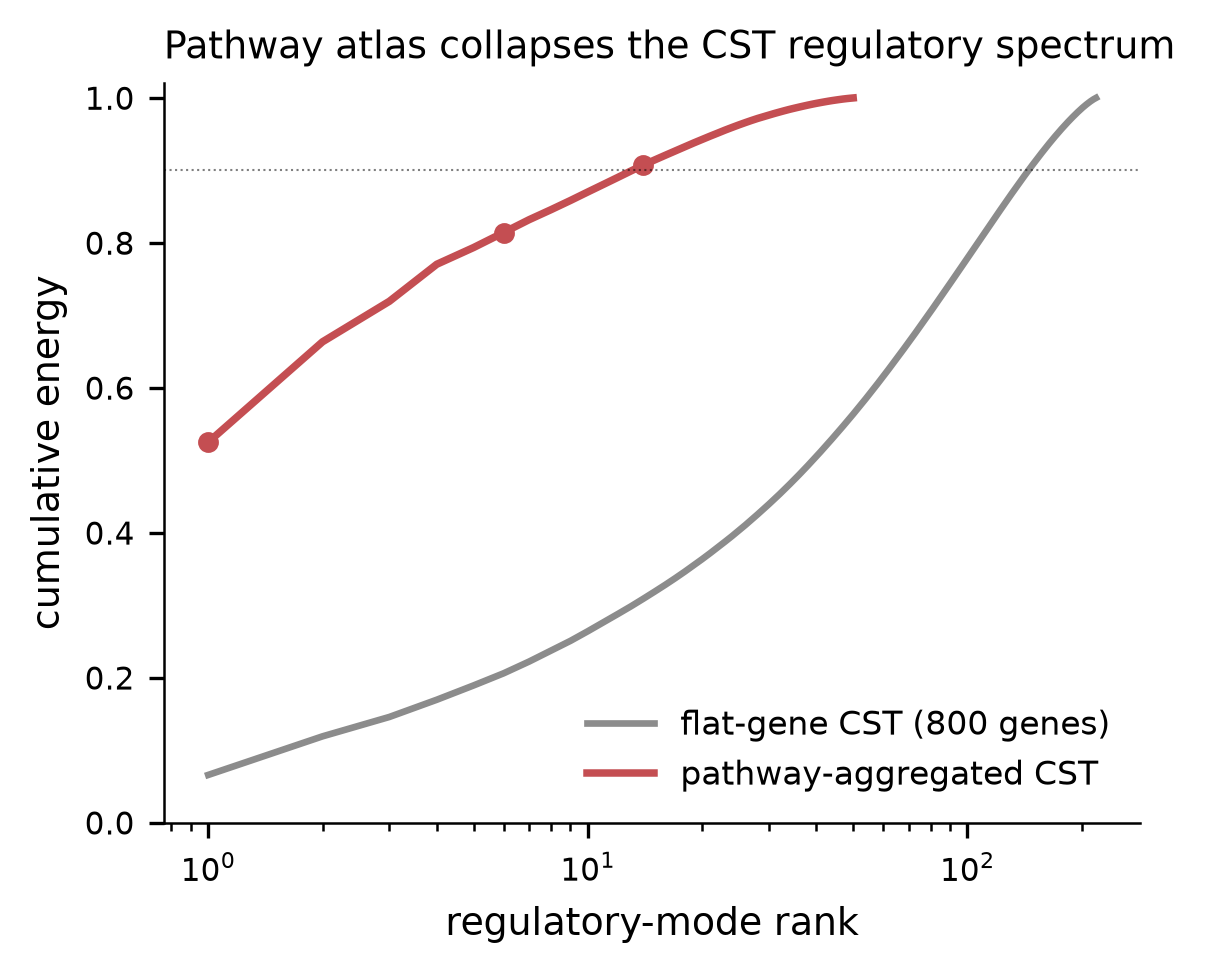
\includegraphics[width=\linewidth]{cst_pathway_spectrum.png}
\caption{Regulatory-mode cumulative energy: the pathway-aggregated CST reaches
$52.5\%$ at rank~$1$; the flat-gene CST needs $\sim\!50$ components for $50\%$.}
\label{fig:cst_pathway_spectrum}
\end{subfigure}\hfill
\begin{subfigure}[t]{0.48\textwidth}
\centering
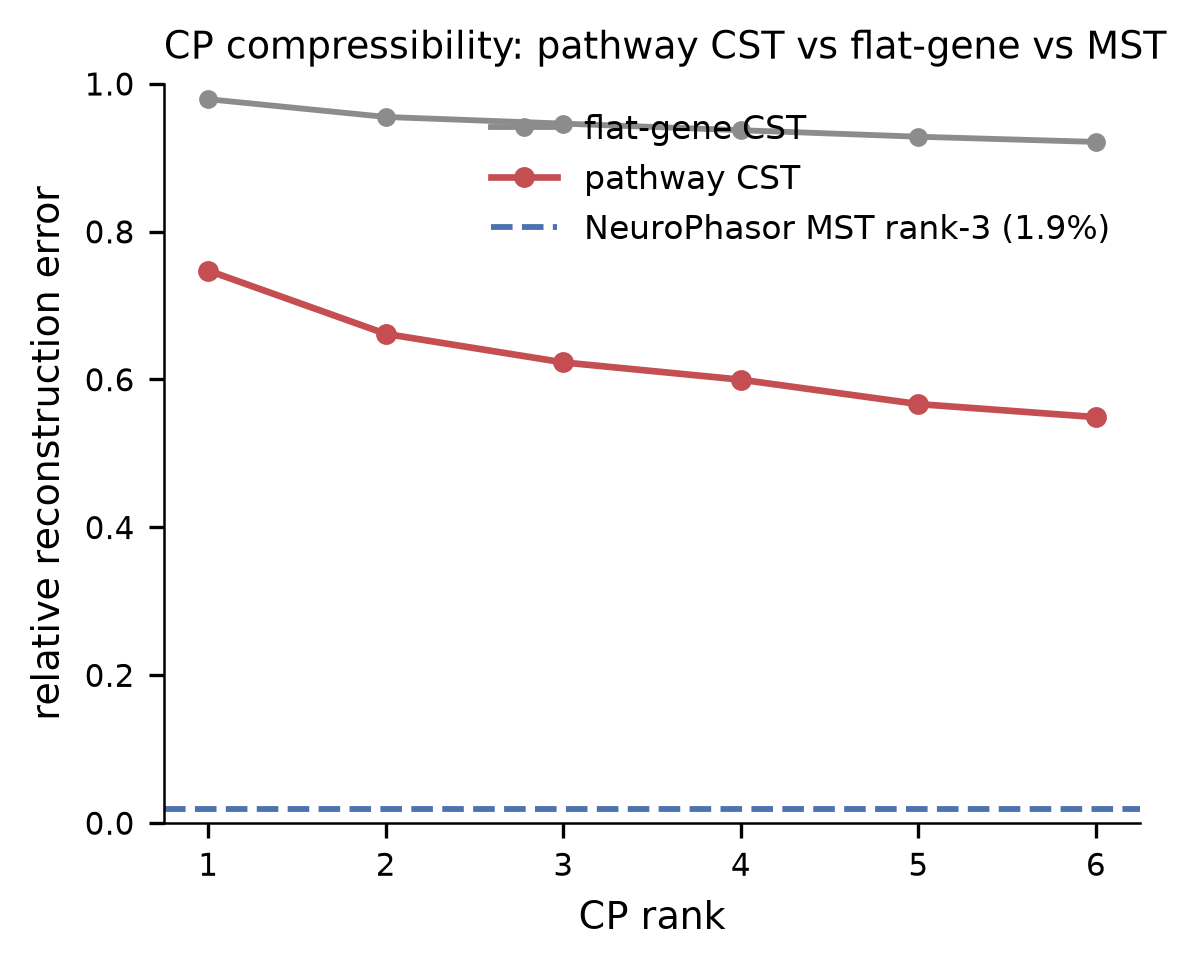
\includegraphics[width=\linewidth]{cst_pathway_cp_error.png}
\caption{CP reconstruction error vs rank: the pathway CST ($62\%$ at rank~3)
beats flat-gene ($95\%$) but does not reach the few-percent regime of a fully
structured tensor (dashed reference).}
\label{fig:cst_pathway_cp}
\end{subfigure}
\caption{\textbf{A pathway atlas roots the CST regulatory axis (real CPTAC
UCEC).} Aggregating $7083$ genes onto $50$ MSigDB Hallmark programs supplies the
regulatory axis with biological structure---the multi-omics counterpart of an
anatomical atlas. \textbf{(a)}~This collapses the regulatory-mode spectrum
toward the low-rank regime; \textbf{(b)}~full-tensor CP compressibility remains
partial because the cohort's sample axis carries irreducible tumour
heterogeneity (see text).}
\label{fig:cst_pathway_fig}
\end{figure}

\begin{figure}[t]
\centering
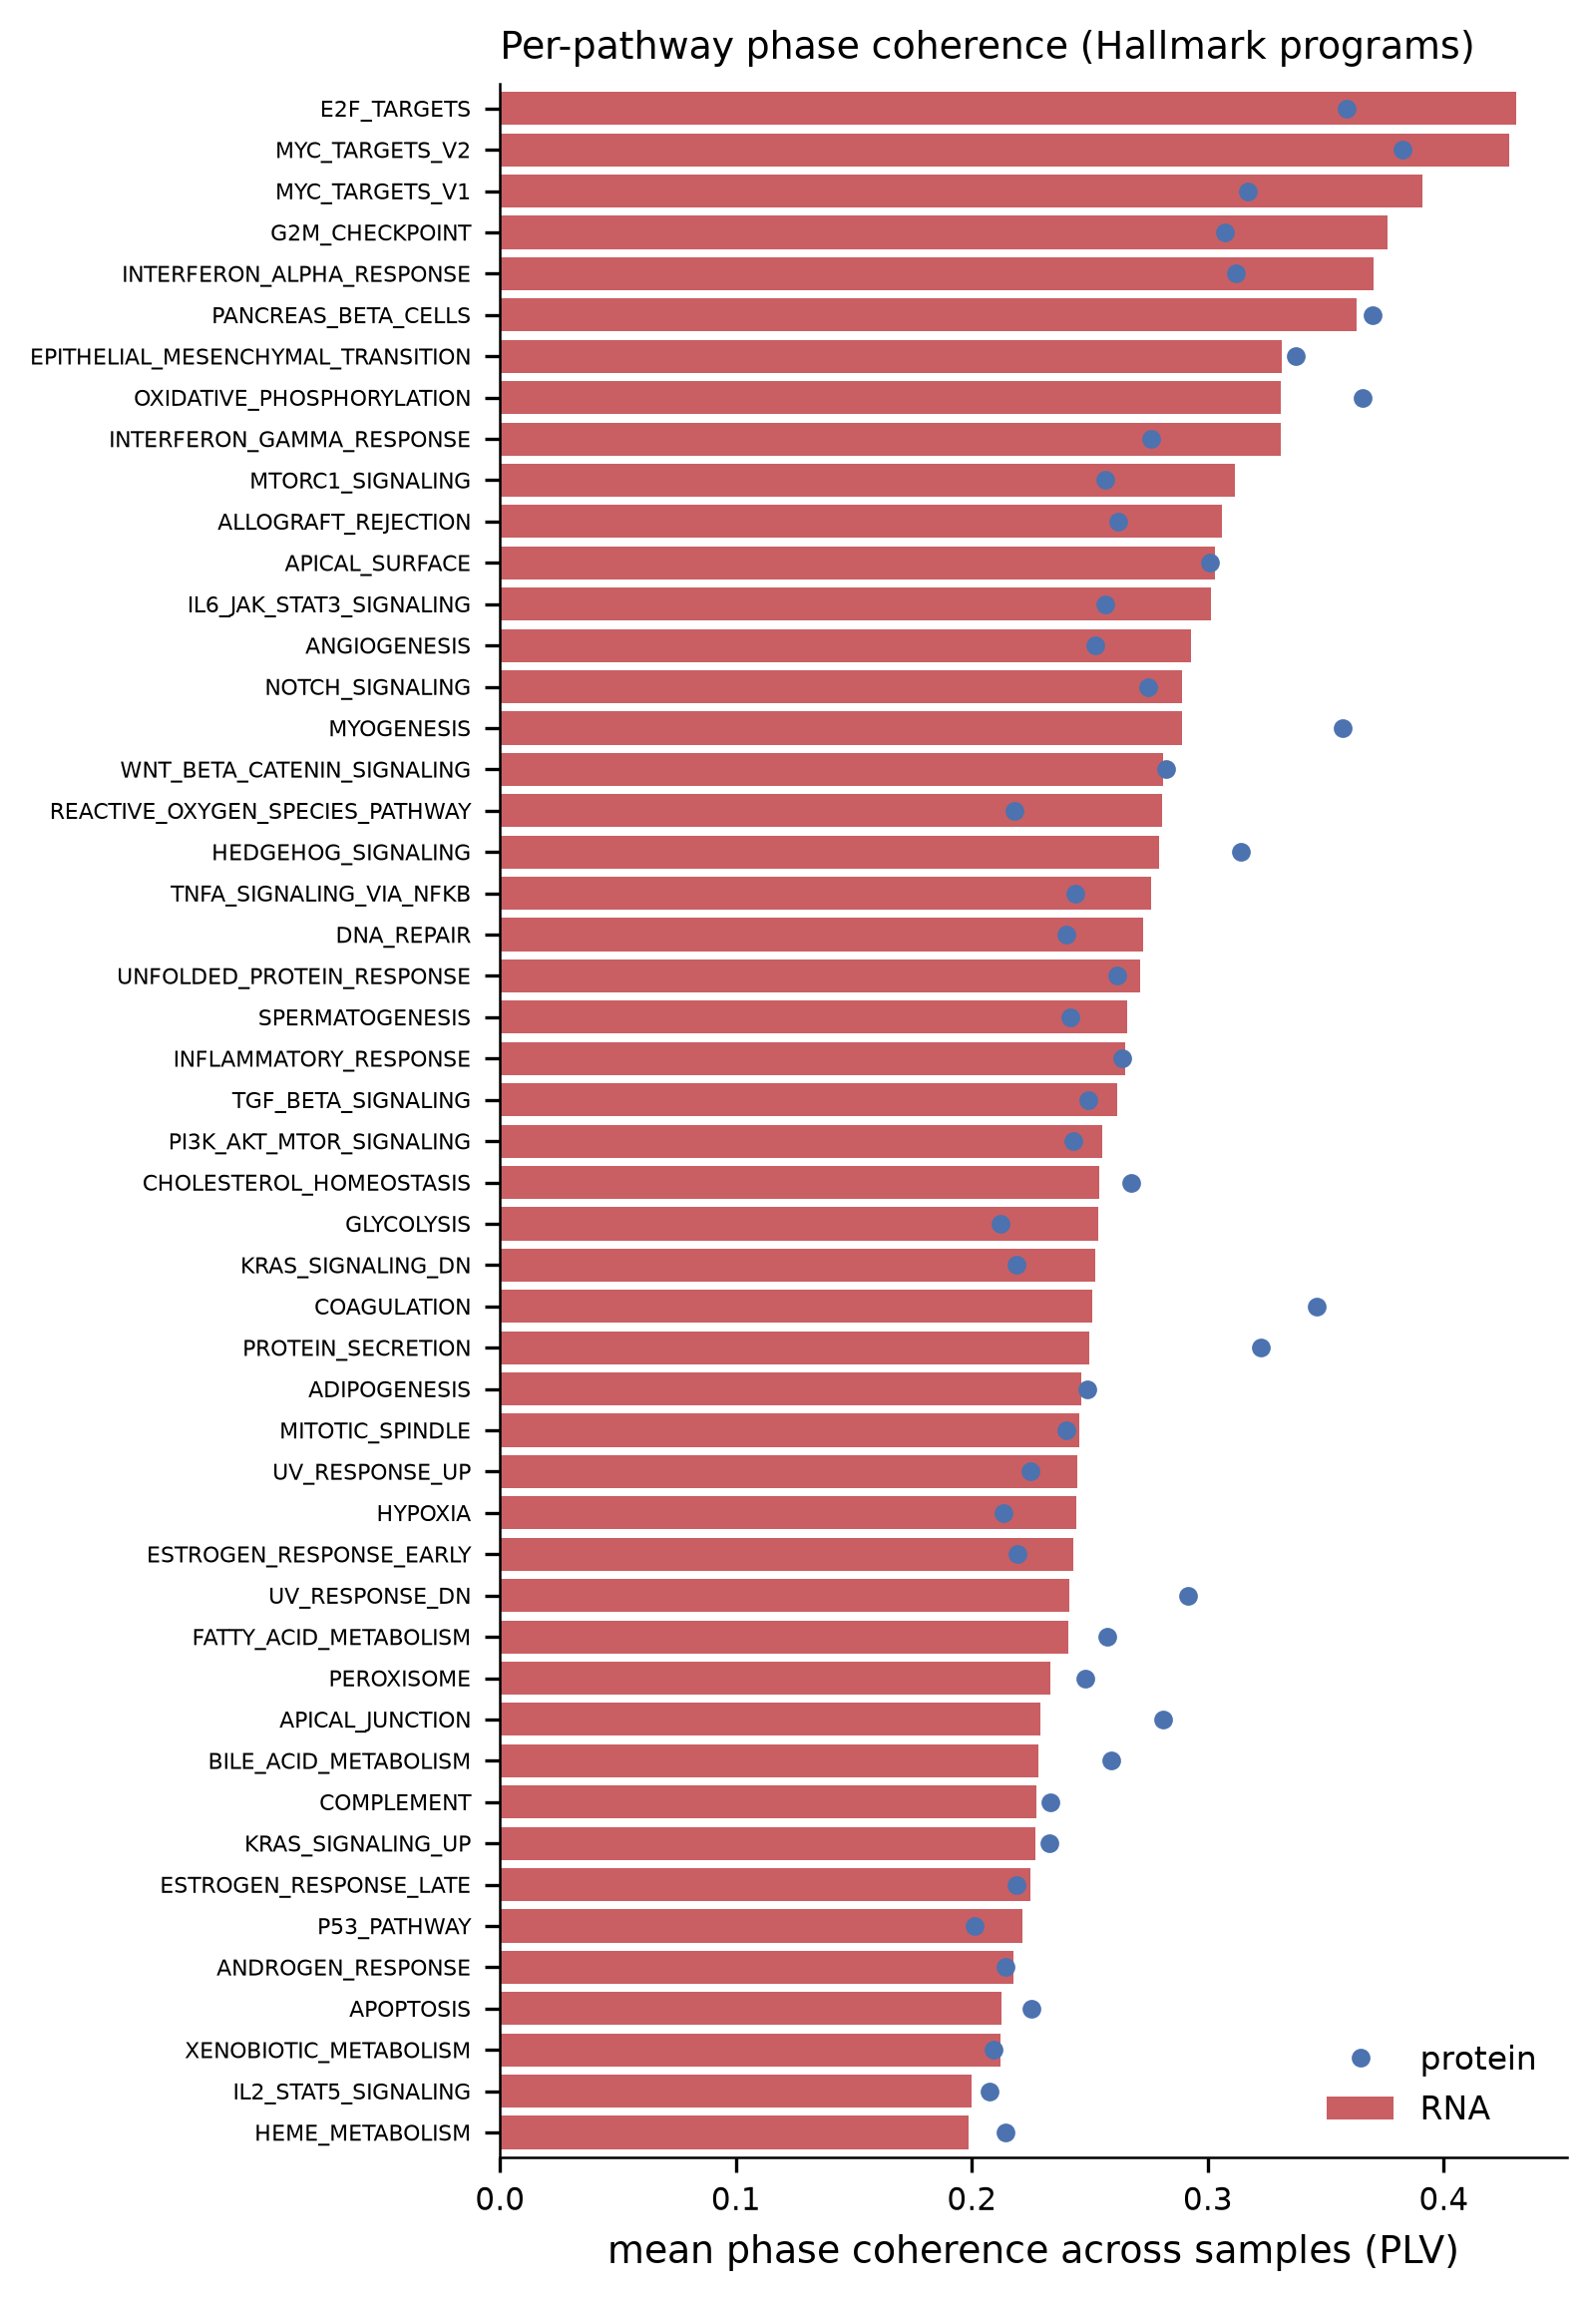
\includegraphics[width=0.62\linewidth]{cst_pathway_coherence.png}
\caption{\textbf{Per-pathway phase coherence across the UCEC cohort.} Mean
across-sample phase coherence (PLV) of each Hallmark program, RNA (bars) and
protein (points). Proliferation programs (\textsc{e2f}, \textsc{myc},
\textsc{g2m}) and \textsc{oxidative\_phosphorylation} are the most phase-coherent;
immune and xenobiotic-metabolism programs the least---an interpretable
biological readout off the pathway atlas, analogous to reading structure off a
brain atlas's regions. Protein coherence is generally lower than RNA, consistent
with post-transcriptional buffering.}
\label{fig:cst_pathway_coherence}
\end{figure}

% ================================================================
\subsection{Central-Dogma Cross-Modal Phase Coupling as a Use Case}
\label{subsec:r_cst_pac}

This is the central result of the paper: a worked use case in which the BioPhasor
formulation---specifically the central-dogma modality axis of the CST---turns a
qualitative expectation about post-transcriptional regulation into a quantitative,
null-calibrated, tumour-specific measurement on real matched multi-omics data. We
develop it in depth: the measurement definition, the effect and its surrogate
null, the per-gene and FDR structure, the regulatory-module organisation, the
tumour-specificity, and the symmetry/directionality question.

\subsubsection{The measurement: phase--amplitude coupling across a modality boundary}

The modality axis (Section~\ref{subsec:cst_measured}) follows the central dogma
(DNA\,$\rightarrow$\,mRNA\,$\rightarrow$\,protein). Cross-frequency
phase--amplitude coupling (PAC), in which the phase of a slow oscillation
organises the amplitude of a faster one, is a standard readout of cross-scale
coordination in neuroscience~\citep{scherer2022}; BioPhasor transposes it from two
frequency bands of one signal onto \emph{two modalities} along a causal axis. For
each gene we bin its across-sample mRNA phase into $K=9$ equal bins, take the mean
protein amplitude in each bin, and score the non-uniformity of that
phase--amplitude histogram with a Tort-style modulation index (MI). Departure from
uniformity means the protein amplitude a gene reaches depends on where its mRNA
sits in phase---a cross-modal coupling. The surrogate null circularly permutes the
sample correspondence \emph{between} modalities ($N=10{,}000$ permutations),
destroying any cross-modal relationship while preserving each modality's own
marginal distribution exactly; this is the correct null because it removes only
the quantity of interest. Because CPTAC is a patient \emph{cohort} rather than a
time course, this is explicitly a \emph{cross-sample} coupling, not a temporal
translation lag---a distinction we return to under directionality.

\subsubsection{The effect clears the surrogate null decisively}

The coupling is present and highly significant
(Fig.~\ref{fig:cst_pac_comod}a,b). At $N=10{,}000$ permutations the aggregate
per-gene MI is $0.0177$ against a null mean of $0.0077$---$z=180$, empirical
$p\approx1\times10^{-4}$, roughly $2.3\times$ the null. A complementary pooled
circular--linear correlation between mRNA phase and protein amplitude gives
$r=0.295$ ($95\%$ bootstrap CI $[0.291,0.299]$), so the two estimators---a
per-gene information-theoretic index and a pooled correlation---agree that a real
cross-modal dependence is present. The comodulogram
(Fig.~\ref{fig:cst_pac_comod}a) shows the shape of it directly: $z$-scored protein
amplitude rises and falls systematically across mRNA-phase bins in tumours, and is
flat in normals.

\subsubsection{The coupling is genome-wide, not a few-gene artefact}

A significant aggregate could in principle be driven by a handful of extreme
genes. It is not. The per-gene modulation-index distribution
(Fig.~\ref{fig:cst_pac_ranking}) is shifted almost in its entirety relative to the
null: $4{,}988$ of $7{,}083$ genes ($70.4\%$) remain individually significant
after Benjamini--Hochberg FDR control at $<0.05$ (raw $p<0.05$: $73.1\%$). The
coupling is thus a genome-wide property of the malignant cohort rather than a
property of a few outliers---a distinction that matters for interpretation, since
a pervasive coupling points to a global regulatory regime rather than a handful of
strongly buffered genes.

\subsubsection{The coupling has coherent regulatory-module structure}

Ranking genes by coupling strength does not return a biologically arbitrary list.
The most strongly coupled genes form a coherent epithelial-polarity /
cell-junction module (\textit{OCLN}, \textit{CXADR}, \textit{MYO5B},
\textit{SLC9A3R1}, \textit{LAD1}, \textit{EPS8}) together with estrogen-signalling
genes (\textit{ESR1}, \textit{ESRP2})---both plausible axes of dysregulation in
endometrial carcinoma. This is where the CST's regulatory axis and its modality
axis meet: the same pathway/module atlas that roots the regulatory axis and makes
the CST compressible (Section~\ref{subsec:r_cst_pathway},
Fig.~\ref{fig:cst_pathway_coherence}) also organises \emph{which} genes couple
most strongly across modalities. The coupling is not spread uniformly over
unrelated genes; it concentrates in interpretable functional programs, which is
the behaviour a regulatory---rather than technical---origin would predict.

\subsubsection{The coupling is a feature of the malignant state}

The coupling is strongly tumour-specific (Fig.~\ref{fig:cst_pac_comod}d): the
pooled circular--linear correlation is $r=0.295$ across the $95$ tumour samples but
only $r=0.029$ across the $14$ normal samples---an order-of-magnitude contrast. A
cross-modal phase--amplitude coupling along the central dogma is therefore not a
generic property of the tissue but something the malignant regulatory state
brings with it. This is the observation that would motivate the coupling as a
candidate axis of tumour biology, and it is the reason this use case is worth a
dedicated study rather than a line in a capability table.

\subsubsection{Is the coupling directional?}

The central dogma is directional, so the natural reading is that mRNA phase
\emph{drives} protein amplitude. We tested this by measuring the reverse
coupling---protein phase organising mRNA amplitude---on the same tumours, and
found it nearly as strong ($r=0.285$ reverse vs.\ $0.295$ forward, a ratio of
$1.04$). At the cohort level the coupling is therefore \emph{symmetric}: the data
establish a real, tumour-specific cross-modal coupling but do \emph{not}
demonstrate a directional mRNA$\to$protein flow (Fig.~\ref{fig:cst_pac_comod}d).
Genuine directionality---a translation lag in which mRNA phase leads protein by a
measurable interval---would require a matched multi-omics \emph{time course},
which a cross-sectional cohort cannot supply. We read the symmetric coupling as
the signature of pervasive post-transcriptional regulation~\citep{srivastava2022},
in which transcript and protein abundances are jointly organised, rather than as
one layer causally setting the other. Stating this plainly is part of the use
case: the phasor formulation makes both the coupling \emph{and} the limit of what
a cohort can say about its direction precise.

\subsubsection{Effect size and scope of the claim}

Two honest caveats bound the result. First, the absolute magnitude is modest
(aggregate MI $\sim\!2.3\times$ the null, pooled $r\approx0.30$): a decisively
significant coupling is not the same as a strong single-gene predictor, and we do
not claim the latter. Second, the normal-sample contrast rests on only $14$
samples, so the order-of-magnitude tumour/normal ratio, while striking, should be
read as motivating rather than definitive. Neither caveat undercuts the core
finding, which is that the coupling clears its surrogate null decisively and
consistently across per-gene, pooled, FDR-controlled, module-structured, and
tumour/normal-stratified views. As a use case it does exactly what a use-case
paper should: it establishes the central-dogma modality axis as a genuine,
non-neural BioPhasor observable equipped with a proper null---the piece that makes
the CST a multi-omics object rather than a phasor tensor by analogy---and it maps
precisely how far the present data license the claim.

\begin{figure*}[t]
\centering
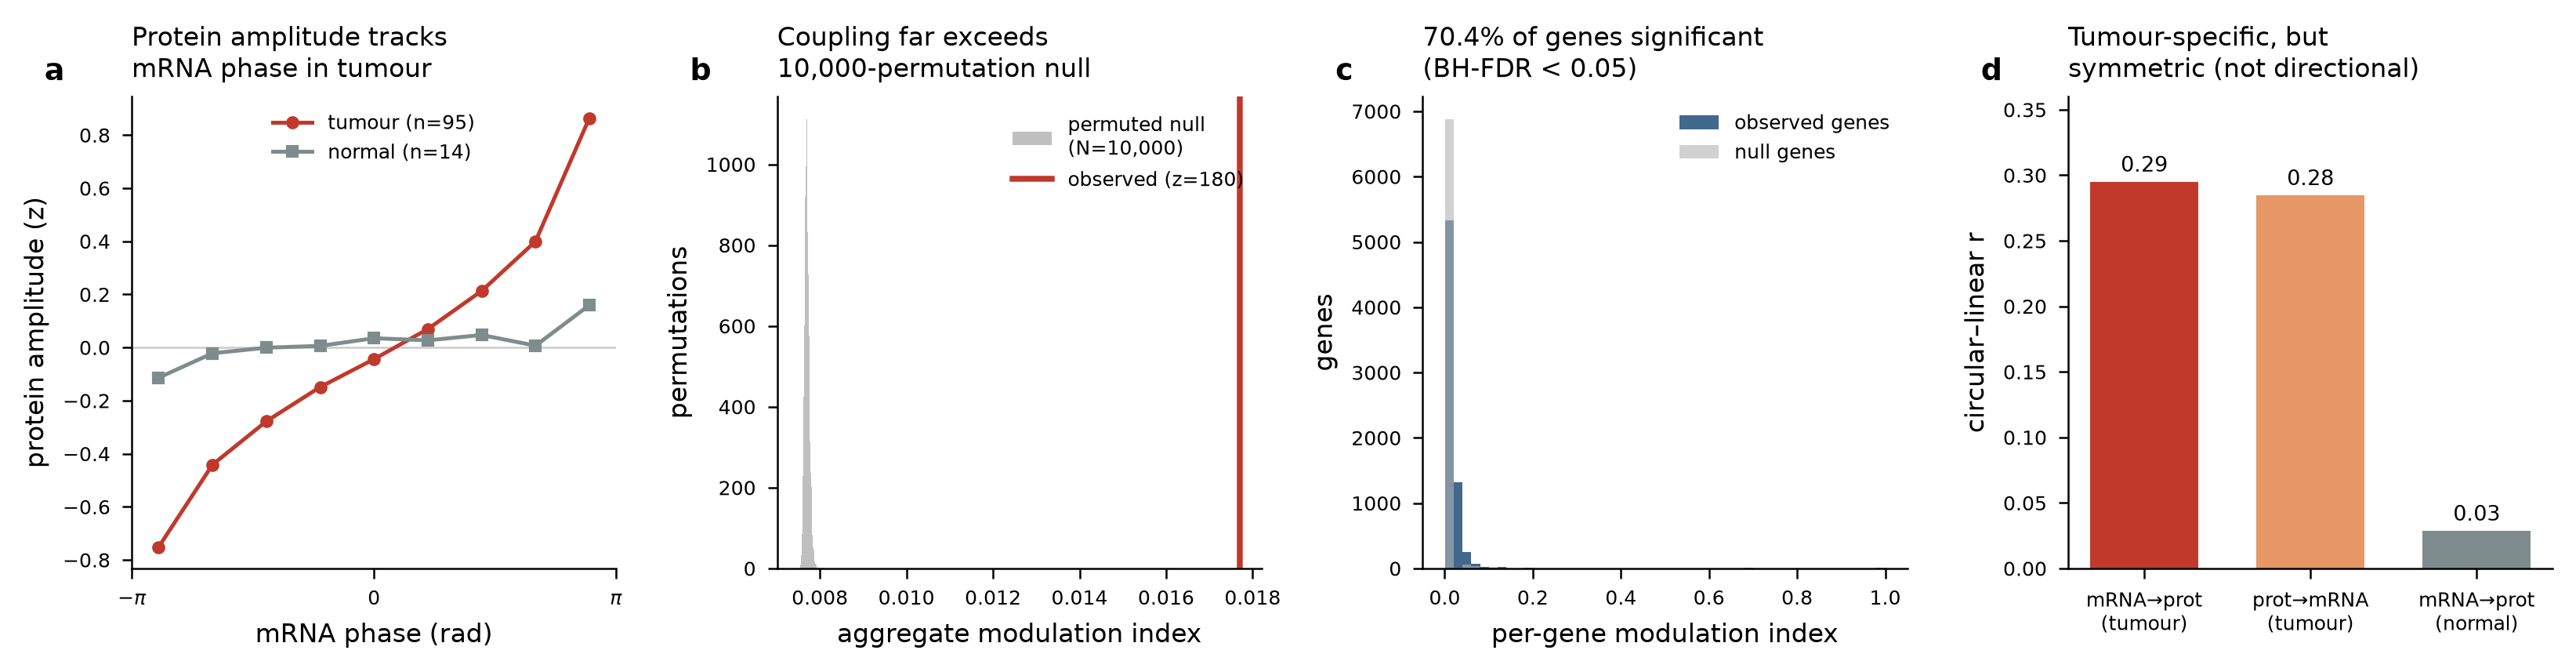
\includegraphics[width=\linewidth]{fig1_omics_pac.png}
\caption{\textbf{Tumour-specific cross-modal phase--amplitude coupling along the
central dogma (real CPTAC UCEC, $109$ patients).} \textbf{(a)}~Comodulogram:
$z$-scored protein amplitude versus mRNA-phase bin, tumours (red) versus normals
(grey); protein amplitude tracks mRNA phase in tumours but not normals.
\textbf{(b)}~Observed aggregate modulation index lies far outside the
$10{,}000$-permutation sample-shuffled null ($z=180$). \textbf{(c)}~Per-gene
modulation-index distribution, observed versus null---$70.4\%$ of genes remain
significant at BH-FDR $<0.05$. \textbf{(d)}~The coupling is tumour-specific
($r=0.29$ vs.\ $0.03$ in normals) but \emph{symmetric}: the reverse
protein$\to$mRNA coupling ($r=0.28$) is nearly as strong as the forward
mRNA$\to$protein coupling ($r=0.29$), so the cohort-level result is not a
demonstration of directional flow.}
\label{fig:cst_pac_comod}
\end{figure*}

\begin{figure}[t]
\centering
\begin{subfigure}[t]{0.48\textwidth}
\centering
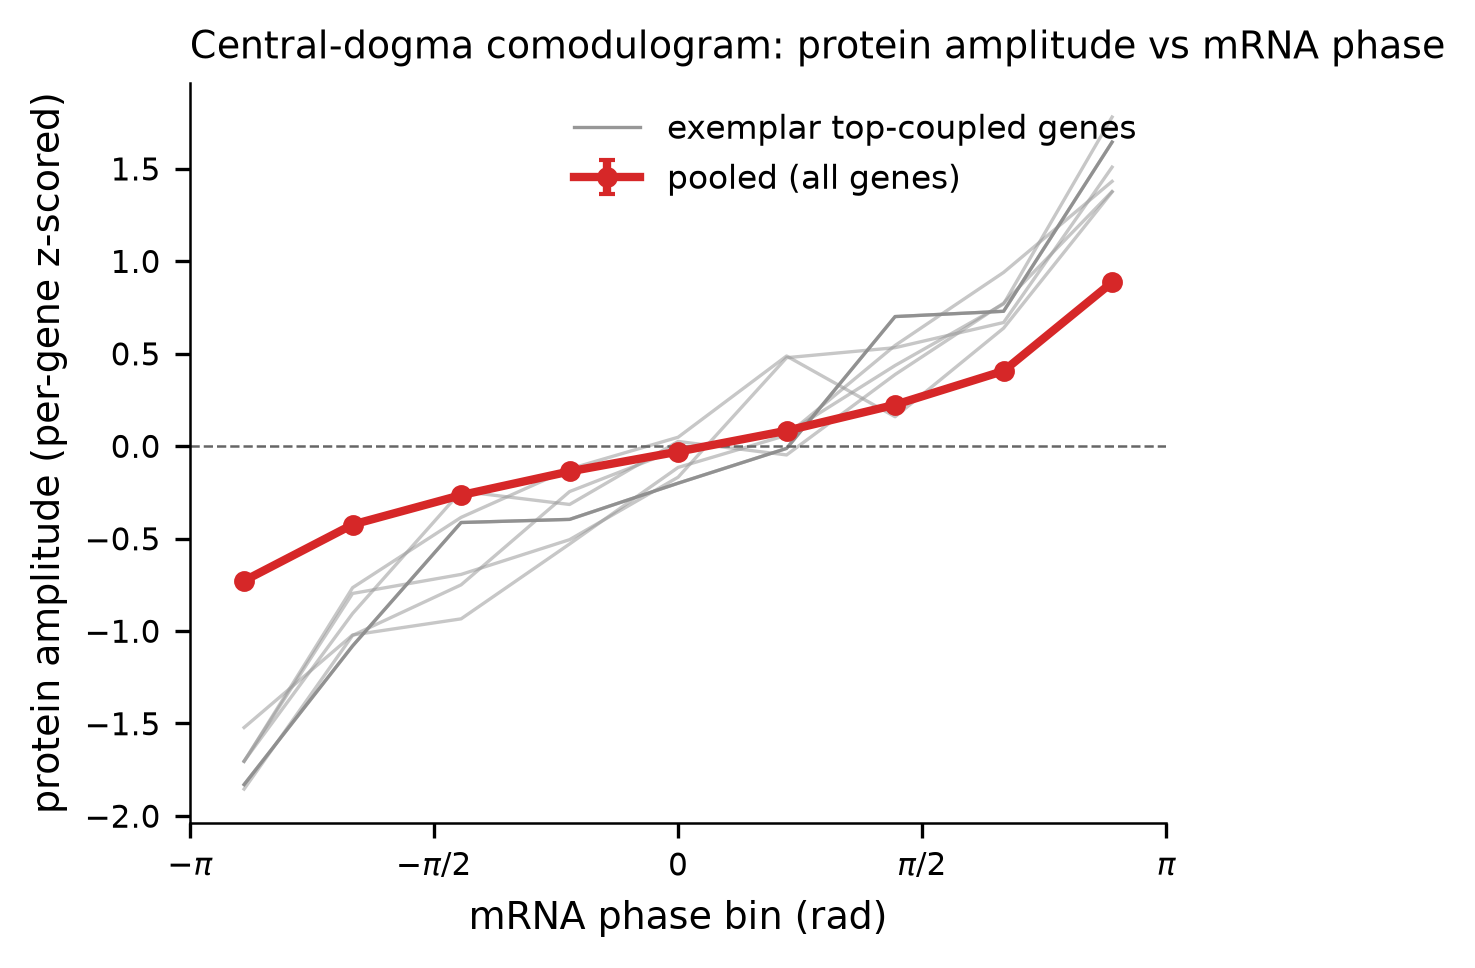
\includegraphics[width=\linewidth]{cst_omics_pac_comodulogram.png}
\caption{Pooled comodulogram (all genes, exemplars light).}
\label{fig:cst_pac_comod_legacy}
\end{subfigure}\hfill
\begin{subfigure}[t]{0.48\textwidth}
\centering
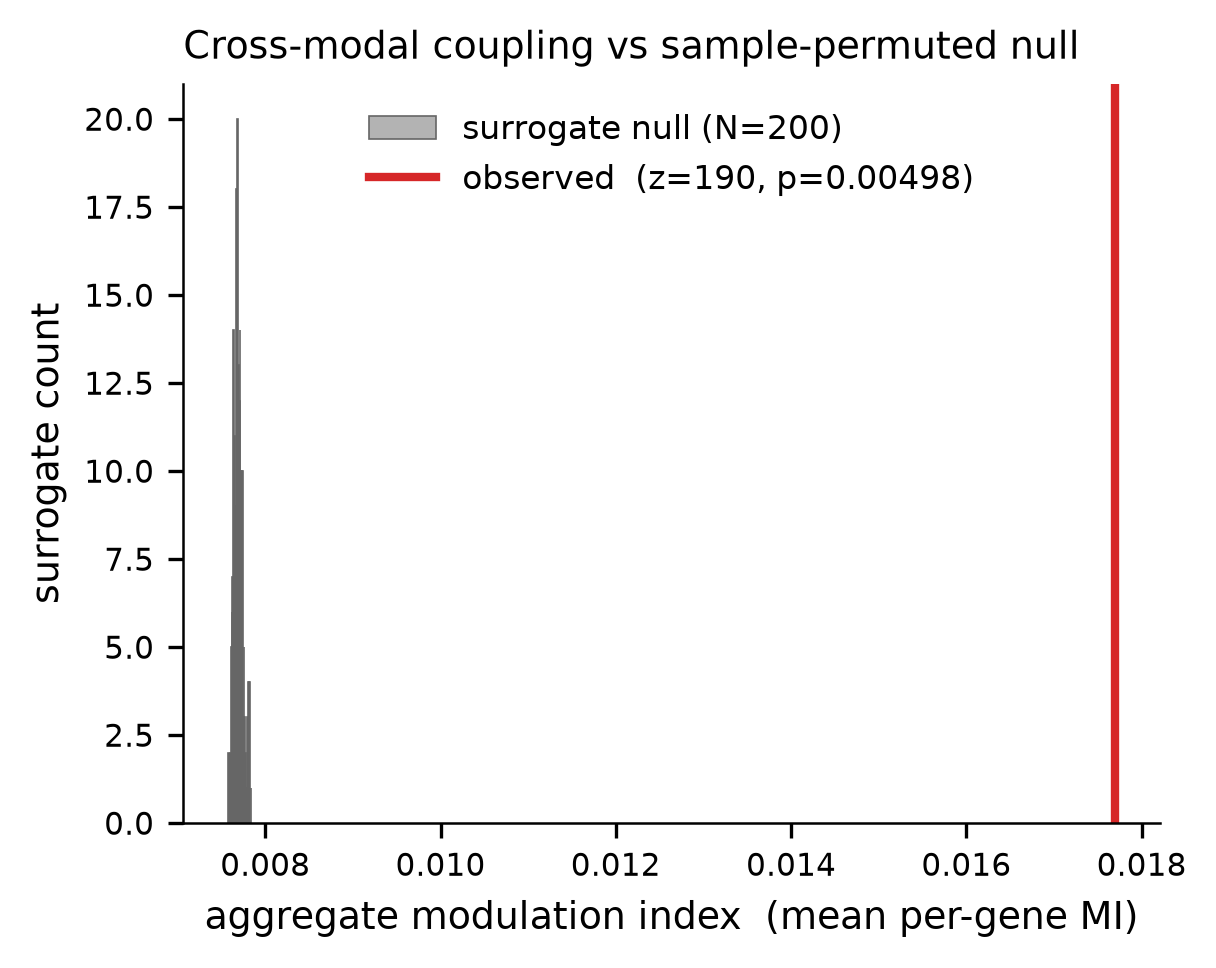
\includegraphics[width=\linewidth]{cst_omics_pac_null.png}
\caption{Observed aggregate MI vs sample-permuted null.}
\label{fig:cst_pac_null}
\end{subfigure}
\caption{\textbf{Supporting per-run views of the central-dogma coupling}
(single-cohort renderings underlying Figure~\ref{fig:cst_pac_comod}).}
\label{fig:cst_pac_fig}
\end{figure}

\begin{figure}[t]
\centering
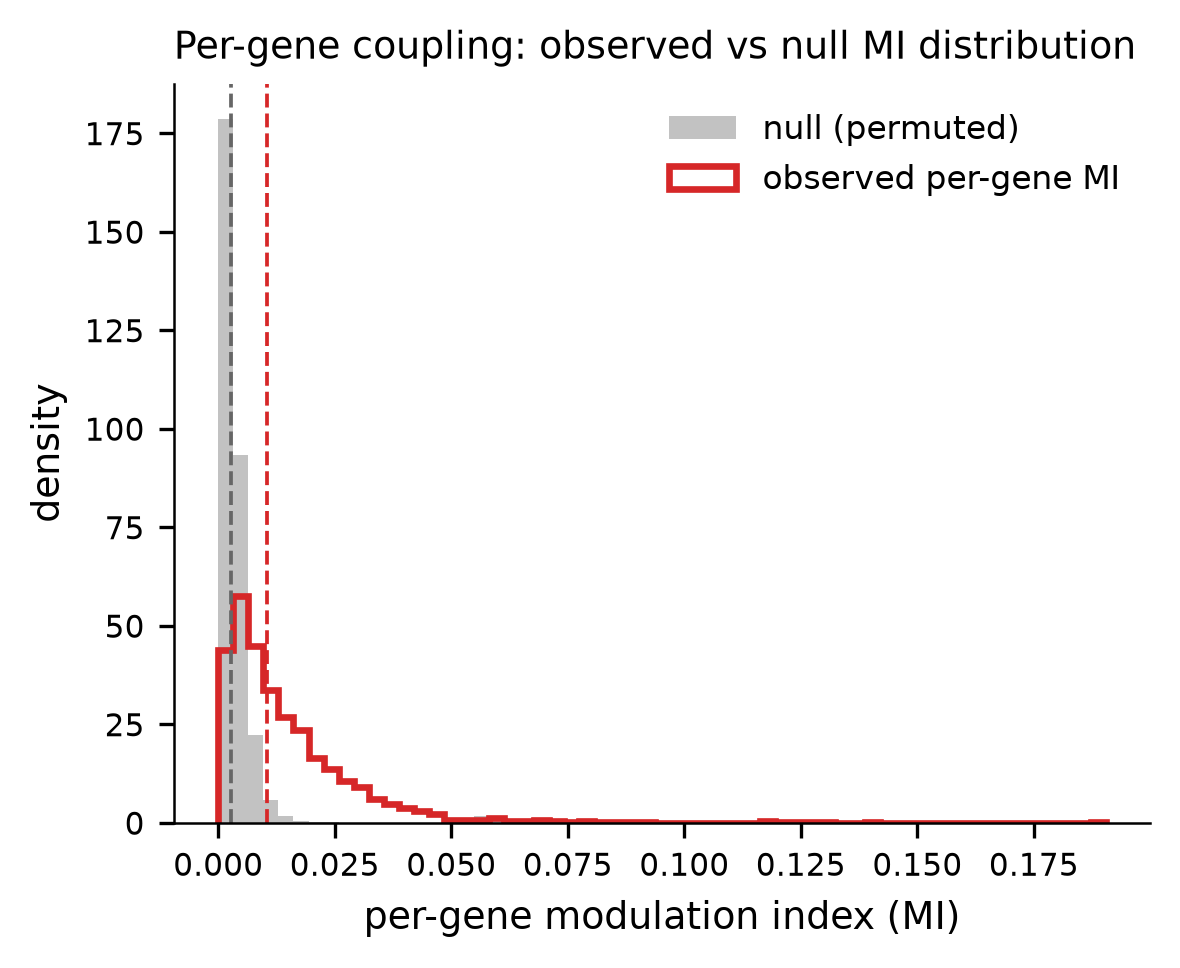
\includegraphics[width=0.62\linewidth]{cst_omics_pac_ranking.png}
\caption{\textbf{Per-gene coupling is broad.} Distribution of per-gene
modulation index, observed (outline) versus sample-permuted null (filled):
$4{,}988/7{,}083$ genes ($70.4\%$) remain significant at BH-FDR $<0.05$
(raw $p<0.05$: $73.1\%$), so the central-dogma coupling is a genome-wide
property of the cohort rather than a few-gene artefact.}
\label{fig:cst_pac_ranking}
\end{figure}

% ================================================================
% ================================================================
\subsection{Data Sources and Reproducibility}
\label{subsec:data_sources}

All results in this draft derive from open, public datasets loaded through
the unmodified BioPhasor \texttt{io} layer (which ingests 10x \texttt{.h5},
\texttt{.h5ad}, MEX, and count/FPKM tables via \texttt{scanpy}/\texttt{anndata}).
Table~\ref{tab:datasources} lists the datasets used across all nine measured
experiments; the same open accessions scale up to the larger cohorts targeted
for the next iteration.

\begin{table*}[t]
\centering
\caption{Public data source for this use-case study. The matched multi-omics
cohort is open-access and the analysis is fully reproducible from a single
loader; the broader dataset panel exercised by the platform is documented in the
companion method paper~\cite{biophasor_platform}.}
\label{tab:datasources}
\begin{tabular}{p{3.4cm}p{1.5cm}p{3.4cm}p{5.8cm}}
\toprule
\textbf{Analysis} & \textbf{Status} & \textbf{Accession / source} & \textbf{Description \& role} \\
\midrule
Pathway atlas + central-dogma coupling
(\S\ref{subsec:r_cst_pathway},\,\S\ref{subsec:r_cst_pac}) & Measured &
CPTAC UCEC (\texttt{cptac}) &
Matched RNA-seq + mass-spec proteomics, same $109$ samples ($95$ tumour,
$14$ normal); regulatory-axis atlas and cross-modal phase--amplitude coupling. \\
\bottomrule
\end{tabular}
\end{table*}

The scRNA-seq and circadian datasets are retrieved directly from the NCBI GEO
FTP mirror; the matched multi-omics cohort (CPTAC UCEC) is retrieved through
the open \texttt{cptac} distribution. A single reproducible loader per
scenario (under \texttt{experiments/codes/}) pulls each dataset, runs it
through the corresponding BioPhasor module at documented defaults, and
regenerates every reported number and figure. No parameter tuning to the
evaluation references was performed---documented defaults (tanh-phase encoding,
canonical marker sets, rhythmicity threshold $0.30$, coherence threshold
$0.30$) were used throughout, and every reference set (scanpy cell-cycle,
literature clock ZTs, pan-essential families) is treated as an external
comparison rather than a tuning target. Verdicts are reported honestly as
reproduces, partial, or does-not-reproduce; the negatives (encoding-coherence
selection, multi-omics fusion, CST knockout screen) are reported in full
because they scope where the framework's operators are valid. One
implementation note affects the tensor-train comparison in
Section~\ref{subsec:r_cst_pathway}: the complex tensor-train SVD in
\texttt{tensorly}~$0.9.0$ is numerically unreliable on our data (its
reconstruction error increases with bond dimension), so every tensor-train
decomposition operates on a real/imaginary-stacked representation of the complex
CST rather than the complex tensor directly.

% --- END sections/results.tex ---

% ================================================================
\section{Discussion}
\label{sec:discussion}

\subsection{What the coupling means biologically}

The result of this study is a single, sharply defined phenomenon: across a
matched tumour cohort, the phase of a gene's mRNA phasor organises the amplitude
of its protein, decisively above a surrogate null, genome-wide, concentrated in
coherent regulatory modules, and specific to the malignant state. The natural
biological reading is post-transcriptional regulation. Transcript and protein
abundances are not related by a fixed proportionality; the efficiency with which
a transcript is translated and the stability of the resulting protein are
themselves regulated---by RNA-binding proteins, microRNAs, codon usage, and
degradation machinery~\citep{srivastava2022}. A phase--amplitude coupling along
the central dogma is exactly the cohort-level footprint such regulation would
leave: the position a gene occupies in transcriptional phase constrains the
protein amplitude it reaches. That the most strongly coupled genes form an
epithelial-polarity / cell-junction module together with estrogen-signalling
genes is consistent with the biology of endometrial carcinoma, where loss of
epithelial organisation and estrogen-driven programs are established axes of
dysregulation; the coupling concentrates where a regulatory---rather than
technical---origin would predict.

The tumour-specificity is the observation that gives the phenomenon its interest.
A coupling that is an order of magnitude stronger in tumours than in matched
normals is not a generic property of the tissue but something the malignant
regulatory state carries. Whether that reflects a global loss of translational
buffering, a rewiring of specific post-transcriptional programs, or both, is a
question this cohort raises rather than answers---but it is a well-posed question
precisely because the phasor formulation renders the coupling measurable and
null-calibrated.

\subsection{Why a phase-geometric measurement}

Existing multi-omics integration methods (MOFA+, similarity network fusion, CCA,
scVI) summarise the joint variation of modalities, but they do not natively
express a \emph{phase}-of-one-modality organising \emph{amplitude}-of-another
relationship: that is a directional, cross-scale coupling of the kind
phase--amplitude coupling was built to quantify in neuroscience. Encoding each
modality as a phasor on $\torus^N$ makes the mRNA ``phase'' and the protein
``amplitude'' first-class, commensurable quantities, and the circular-statistics
machinery supplies both the modulation index and the sample-permuted null that
calibrates it. The measurement is thus not a re-description of correlation but a
quantity that a magnitude-space embedding does not expose. The full formulation
that makes this possible---the encoding, the circular and Riemannian statistics,
and the Cell State Tensor whose modality axis this coupling lives on---is
developed in the companion method paper~\cite{biophasor_platform}.

\subsection{Limitations}

Three limitations bound the claim, and we state them plainly because scoping is
part of the contribution.

\begin{itemize}
  \item \textbf{Effect size.} The coupling is decisively significant but modest in
  magnitude (aggregate modulation index $\sim\!2.3\times$ the null, pooled
  $r\approx0.30$). It is a real, pervasive organising relationship, not a strong
  single-gene predictor, and we do not present it as the latter.
  \item \textbf{Direction is not established.} At the cohort level the coupling is
  symmetric (reverse/forward ratio $1.04$), so a cross-sectional cohort cannot
  demonstrate a translational mRNA$\to$protein flow. Genuine directionality---a
  measurable translation lag---requires matched multi-omics \emph{time series},
  which we identify as the decisive next experiment.
  \item \textbf{Cohort size and scope.} The tumour/normal contrast rests on $14$
  normal samples, and the analysis is one tumour type (CPTAC UCEC). The
  order-of-magnitude tumour-specificity is motivating rather than definitive, and
  generalisation across tumour types (additional CPTAC/TCGA cohorts) is future
  work.
\end{itemize}

None of these undercuts the core finding---a null-calibrated, genome-wide,
tumour-specific cross-modal coupling---but each marks the boundary of what the
present data license.

\subsection{This use case in the BioPhasor series}

BioPhasor is a platform intended to host a series of use-case studies that share
one formulation and one codebase~\cite{biophasor_platform}. This paper is the
first: it develops the central-dogma modality axis of the CST into a
tumour-specific coupling measurement. Companion use cases under development apply
the same formulation to different questions---a spectral connectome reading of the
regulatory axis, and port-Hamiltonian dynamics of the phasor state---each building
on the shared encoding, statistics, and tensor rather than re-deriving them. The
value of the platform model is exactly this separability: the method is
established once, and each use case can then go deep on a single biological
question, as this one does on cross-modal coupling in cancer. The immediate
extension of \emph{this} use case is a matched multi-omics time course, which
would convert the symmetric cohort-level coupling into a directional test of
translational timing, and a pan-cancer sweep to establish whether the
tumour-specific coupling is a general feature of the malignant state.

\section{Conclusion}

Using the BioPhasor formulation~\cite{biophasor_platform}, we have made a single
biological relationship measurable as a first-class, null-calibrated quantity: a
cross-modal phase--amplitude coupling along the central dogma, in which the phase
of a gene's mRNA phasor organises the amplitude of its protein. Across a matched
CPTAC endometrial-carcinoma cohort the coupling clears a stringent
sample-permuted null decisively ($z=180$; pooled circular--linear $r=0.295$), is
genome-wide ($70.4\%$ of $7{,}083$ genes significant at BH-FDR $<0.05$),
concentrates in coherent epithelial-polarity and estrogen-signalling modules, and
is strongly tumour-specific ($r=0.295$ in tumours vs.\ $0.029$ in normals). We
have also drawn the boundary of the claim honestly: the coupling is symmetric at
the cohort level, so these cross-sectional data establish the coupling but not a
directional translational flow---the decisive next experiment is a matched
multi-omics time course, and the natural extension is a pan-cancer sweep.

The broader point is methodological. Post-transcriptional regulation is exactly
the kind of cross-scale, directional relationship that a magnitude-space
integration does not natively express, and that a phase-geometric representation
does. By encoding each modality as a phasor and reading the coupling with the
circular-statistics machinery and its surrogate null, BioPhasor turns a
qualitative expectation into a quantitative, reproducible measurement. This is
the first use-case study built on the shared BioPhasor platform; the formulation
is established once in the companion method paper, and further use cases---a
spectral connectome reading of the regulatory axis, port-Hamiltonian dynamics of
the phasor state---build on the same code and the same geometry rather than
re-deriving them.

\bibliographystyle{unsrt}
\bibliography{references}

\end{document}
